\section{Chart::Composite}
\herv{Name:} Chart::Composite\\ \\
\herv{File:} Composite.pm\\ \\
\herv{Requires:}Chart::Base, GD, Carp, FileHandle\\ \\
\herv{Description:} \fett{Composite} is a \fett{subclass} of Chart::Base.\\
The class Composite creates a two component chart with two types of chart. For example you can create a two component chart with bars and lines. Just set the option 'composite\_info'! A composite chart doesn't make sense with all types of chart. But it works pretty good with Lines, Points, LinesPoints and Bars.\\ 
\\
\herv{Example:}
\begin{figure}[h]
	\begin{center}
		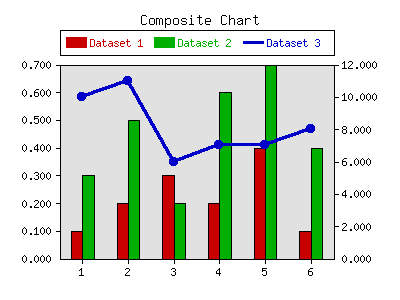
\includegraphics[scale=0.6]{composite.png}
	\end{center}
	\caption{Composite chart}
	\label{fig:composite}
\end{figure}
\begin{verbatim}
use Chart::Composite;

$g = Chart::Composite->new;

$g->add_dataset (1 , 2, 3, 4, 5, 6);
$g->add_dataset (0.1, 0.2, 0.3, 0.2, 0.4, 0.1);
$g->add_dataset (0.3, 0.5, 0.2, 0.6, 0.7, 0.4);
$g->add_dataset (10, 11, 6, 7, 7, 8);

$g->set('title' => 'Composite Chart',
        'composite_info' => [ ['Bars', [1,2]],
                               ['LinesPoints', [3]] ] );
$g->set( 'include_zero' => 'true');

$g->png("composite.png");
\end{verbatim}
\herv{Constructor:} An instance of a Composite object can be created with the constructor new():\\
\fett{\$obj = Chart::Composite->new();}\\
\fett{\$obj = Chart::Composite->new(\kursiv{width}, \kursiv{height});}\\
\\
If \fett{new} has no arguments, the constructor returns an image with the size 300x400 pixels. If new has two arguments \kursiv{width} and \kursiv{height}, it returns an image with the desired size. \\ 
\\ 
\herv{Methods:}All universally valid methods, see page \pageref{methods}: Chart::Base. \\
\\
\herv{Attributes/Options:} All universally valid options, see page \pageref{options}. Also available, these special options:
\begin{description}
\item['composite\_info']This option is only used for composite charts.  It contains the information about which types to use for the two component charts, and which datasets belong to which component chart. It should be a reference to an array of array references, containing information like the following\\
\$obj->set ('composite\_info' => [ ['Bars', [1,2]],                      ['Lines', [3,4] ] ]);\\
\\
This example would set the two component charts to be a bar chart and a line chart. It would use the first two data sets for the bar chart (note that the numbering starts at 1, not zero like most of the other numbered things in Chart), and the second two data sets for the line chart. The default is undef.\\
\\
NB. Chart::Composite can only do two component charts.
\item['min\_val1', 'min\_val2']Only for composite charts, these options specify the minimum y-value for the first and second components respectively. Both default to undef.
\item['max\_val1', 'max\_val2']Only for composite charts, these options specify the maximum y-value for the first and second components respectively. Both default to undef.
\item['y\_ticks1', 'y\_ticks2']The number of y ticks to use on the first and second y-axis on a composite chart.  Please note that if you just set the 'y\_ticks' option, both axes will use that number of y ticks. Both default to undef.
\item['same\_y\_axes']Forces both component charts in a composite chart to use the same maximum and minimum y-values if set to 'true'. This helps to keep the composite charts from being too confusing. Default is undef.
\end{description}